%\title{EMC LaTeX Portrait Poster Template}
%%%%%%%%%%%%%%%%%%%%%%%%%%%%%%%%%%%%%%%%%
% a1poster Portrait Poster
% LaTeX Template
% Version 2.0 (22/06/16)
%
% The a1poster class was created by:
% Joe Rowing (JoeRowing@exeterms.ac.uk)
% 
% This template has been produced by:
% Joe Rowing at Exeter Mathematics School
%
% License:
% CC BY-NC-SA 3.0 (http://creativecommons.org/licenses/by-nc-sa/3.0/)
%
%%%%%%%%%%%%%%%%%%%%%%%%%%%%%%%%%%%%%%%%%

%----------------------------------------------------------------------------------------
%   PACKAGES AND OTHER DOCUMENT CONFIGURATIONS
%----------------------------------------------------------------------------------------

\documentclass[a1,portrait]{a1poster}

\usepackage{multicol} % This is so we can have multiple columns of text side-by-side
\columnsep=50pt % This is the amount of white space between the columns in the poster
\columnseprule=0.01pt % This is the thickness of the black line between the columns in the poster

\usepackage[svgnames]{xcolor} % Specify colors by their 'svgnames', for a full list of all colors available see here: http://www.latextemplates.com/svgnames-colors

\usepackage{times} % Use the times font

\usepackage{graphicx} % Required for including images
\graphicspath{{figs/}} % Location of the graphics files
\usepackage{booktabs} % Top and bottom rules for table
\usepackage[font=small,labelfont=bf]{caption} % Required for specifying captions to tables and figures
\usepackage{amsfonts, amsmath, amsthm, amssymb} % For math fonts, symbols and environments
\usepackage{wrapfig} % Allows wrapping text around tables and figures
\usepackage{hyperref}
\usepackage[epsilon, tsrm, altpo]{backnaur}
\usepackage{listings}
\usepackage{paracol}
\lstset{language=Haskell, upquote=true, stringstyle=\ttfamily, showstringspaces=true}

% https://tex.stackexchange.com/questions/450226/how-to-avoid-column-vertical-line-inside-multicol-environment
\setlength{\columnseprule}{0pt}
\captionsetup{font=large}

\newcommand{\tbcell}[2][0.18]{\includegraphics[width=#1\linewidth, trim={0.1cm 3cm 0.1cm 2.5cm}, clip]{#2}}


\begin{document}

%----------------------------------------------------------------------------------------
%   POSTER HEADER 
% The header is divided into two boxes:
% The first is 75% wide and houses the title, subtitle, names, university/organization and contact information
% The second is 25% wide and houses the EMS Logo
% 
%----------------------------------------------------------------------------------------


\begin{minipage}[b]{0.6\linewidth}
\huge \color{DarkRed} \textbf{Quick and Reusable Code Generation for Idris} \color{Black}\\ % Title
\huge\textit{Integrating dependent types into the industrial services}\\[1cm] % Subtitle
\large \textbf{Taine Zhao \& Yukiyoshi Kameyama}\\[0.5cm] % Author(s)
\large Computer Science, University of Tsukuba \\[0.2cm] % University/organization
\texttt{thaut@logic.cs.tsukuba.ac.jp; kam@cs.tsukuba.ac.jp}\\
\end{minipage}
%
\vspace{.5cm} % A bit of extra whitespace between the header and poster content

%----------------------------------------------------------------------------------------

\begin{multicols}{2} % This is how many columns your poster will be broken into, by convention a portrait poster is generally split into 2 or 3 columns

%----------------------------------------------------------------------------------------
%   ABSTRACT

%An abstract is a brief summary of a research article, thesis, review, conference proceeding or any in-depth analysis of a particular subject and is often used to help the reader quickly ascertain the paper's purpose
%----------------------------------------------------------------------------------------

% \color{CornflowerBlue} % Colour for the abstract

\section*{Abstract}

As a dependently-typed functional programming language, Idris shows
quite a high expressiveness with its type system under a considerably strong static guarantee,
which is capable of ending many difficult and frequently occurring bugs in the industrial world.

To leverage its powerful static programming language features and make
existing industrial applications safer and more expressive,
a valid approach is to implement code generation back ends for Idris.

Whereas Idris has already provided convenient interfaces to support
agnostic back ends, it is still cumbersome to import Idris programs
into an existing programming language. As the existing programming languages are already
in a large amount and continuously proliferating, and the implementations
of different back ends certainly have quite a few overlaps.
  
To address this, we introduce a "common" intermediate representation, Weakest Declaration,
which is a much simpler IR and contributes to reusability of analyses and transformations
required by different Idris back ends.

As a result, we allow making an Idris back end in a most simplified routine,
which can usually be accomplished in few hours or, even minutes.

%----------------------------------------------------------------------------------------
%   INTRODUCTION

%Avoid using technical definitions unless absolutely necessary. The introduction section is here to introduce your issue, so be sure to not bore your readers right away with excessive information. You can even include graphics if they will help the viewer understand the work that you have done.
%----------------------------------------------------------------------------------------

% \color{OrangeRed} % color for the introduction

\section*{Background}

% \includegraphics[width=15cm]{Idris-Backend-For-Free.png}\\
Idris is a programming language with dependent types,
hence it is capable of ending many difficult and frequently occurring bugs in the industrial world:
For instance, dependently typed programs can statically verify the validness of array indexing \cite {xi1998eliminating},
or statically verify the validness of tensor operations \cite {eaton2006statically} \cite {chen2017typesafe},
especially statically checking/inferring dimensions.

\begin{minipage}[b]{1\linewidth}
\begin{center}
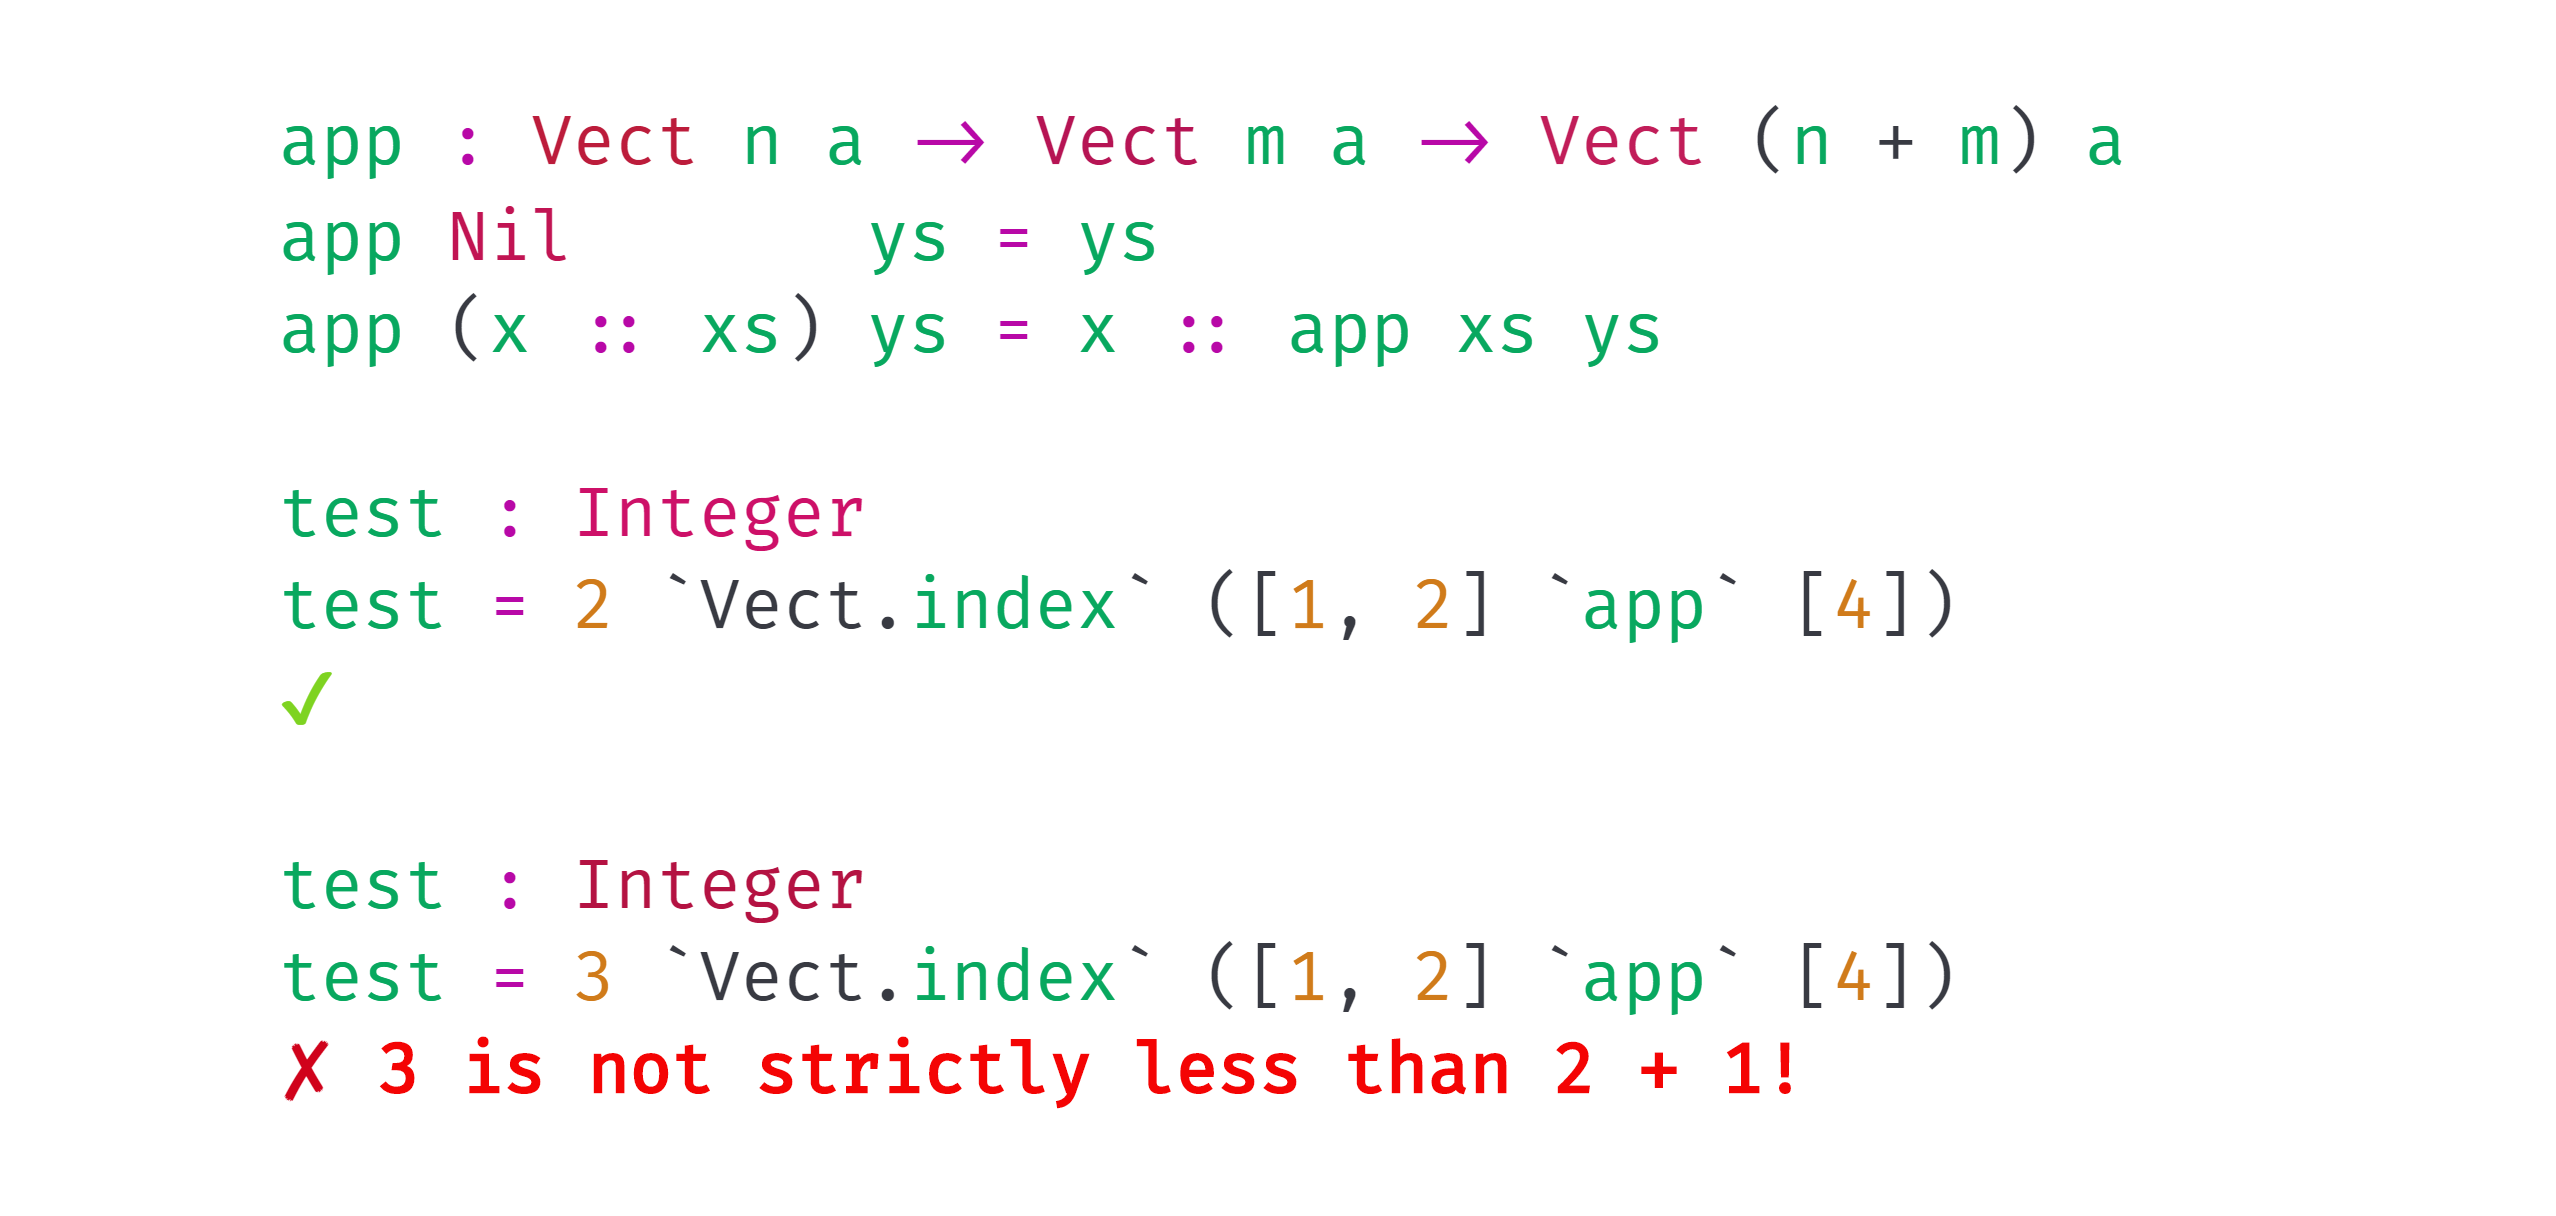
\includegraphics[width=0.8\linewidth]{figs/canonical.png}
\vspace{-1cm}
\captionof{figure}{\color{DarkRed} Canonical example, a dependent vector}
\end{center}

\end{minipage}

\vspace{0.5cm}

To leverage its advanced type system in practice, a valid approach is
implementing code generation back ends for Idris, and integrating Idris into
the existing applications.

To achieve this, Idris has already paid lots of efforts to their code generation facilities,
and finally provided a convenient interface for back end plugins \cite{brady2015cross}.

We hereby provide the definition of Idris defunctionalised IR with some details omitted and simplifications,
hereafter as $DDecl$.

\vspace{-1cm}

\begin{multicols}{2}
\vspace{-1.0cm}
\begin{minipage}[b]{0.8\linewidth}
\begin{bnf*}
    \bnfprod{expr}{\bnftd{Var} \bnfsp \bnftd{name}}\\
    \bnfmore{\bnfor \bnftd{App} \bnfsp \bnftd{bool} \bnfsp \bnftd{name} \bnfsp \bnfts{[} \bnftd{expr}\bnfts{]}}\\
    \bnfmore{\bnfor \bnftd{Let} \bnfsp \bnftd{name} \bnfsp \bnftd{expr} \bnfsp \bnftd{expr}}\\
    \bnfmore{\bnfor \bnftd{Update} \bnfsp \bnftd{name} \bnfsp \bnftd{expr}}\\
    \bnfmore{\bnfor \bnftd{Proj} \bnfsp \bnftd{expr} \bnfsp \bnftd{int}}\\
    \bnfmore{\bnfor \bnftd{Cons} \bnfsp \bnftd{name} \bnfsp \bnfts{[} \bnftd{expr}\bnfts{]}}\\
    \bnfmore{\bnfor \bnftd{Case} \bnfsp \bnftd{expr} \bnfsp \bnfts{[} \bnftd{alt}\bnfts{]}}\\
    \bnfmore{\bnfor \bnftd{Const} \bnfsp \bnftd{constant}}\\
    \bnfmore{\bnfor \bnftd{Foreign} \bnfsp \bnftd{...}}\\
    \bnfmore{\bnfor \bnftd{Op} \bnfsp \bnftd{primitive-op} \bnfsp \bnfts{[} \bnftd{expr}\bnfts{]}}\\
    \bnfmore{\bnfor \bnftd{DoNothing}}\\
    \bnfmore{\bnfor \bnftd{Error} \bnfsp \bnftd{string}}\\
\end{bnf*}
\end{minipage}

\begin{minipage}[b]{1\linewidth}
\begin{bnf*}
    \bnfprod{decl}{\bnftd{DefFun} \bnfsp \bnftd{name} \bnfsp \bnfts{[} \bnftd{name}\bnfts{]} \bnfsp \bnftd{expr}}\\
    \bnfmore{\bnfor \bnftd{DefCons} \bnfsp \bnftd{name} \bnfsp \bnftd{int}}\\
    \bnfprod{alt}{\bnftd{ConCase} \bnfsp \bnftd{name} \bnfsp \bnfts{[} \bnftd{name}\bnfts{]} \bnfsp \bnftd{expr}}\\
    \bnfmore{\bnfor \bnftd{ConstCase} \bnfsp \bnftd{constant} \bnfsp \bnftd{expr}}\\
    \bnfmore{\bnfor \bnftd{DefaultCase} \bnfsp \bnftd{expr}}\\
    \bnfprod{arith-type}{\bnftd{float} \bnfor \bnftd{int}}\\
    \bnfprod{primitive-op}{\bnftd{+} \bnfsp \bnftd{arith-type}}\\
    \bnfmore{\bnfor \bnftd{-} \bnfsp \bnftd{arith-type}}\\
    \bnfmore{\bnfor \bnftd{*} \bnfsp \bnftd{arith-type}}\\
    \bnfmore{\bnfor \bnftd{sdiv} \bnfsp \bnftd{arith-type}}\\
    \bnfmore{\bnfor \bnftd{udiv} \bnfsp \bnftd{arith-type}}\\
    \bnfmore{\bnfor \bnftd{...}}\\
\end{bnf*}
\end{minipage}
\vspace{-1cm}
\end{multicols}
\vspace{-1.5cm}
\begin{center}  \textbf{Language 1}: \color{DarkRed} \textbf{Defunctionalised Declarations} \end{center}

\begin{itemize}
    \setlength\itemsep{-0.38em}
    \item $Cons$, $DefCons$ : constructing tagged unions, and constructor definitions
    \item $Case$ : pattern matching, or deconstructions
    \item $Proj$ : projections, on tuples and tagged unions
    \item $primitive$-$op$ : $+$, $-$, $*$, $/$, and other primitive operators defined and used by Idris compiler
\end{itemize}

\captionsetup{font=normalsize}

\vspace {-0.5cm}
\section*{Investigation}

$DDecl$ is already convenient for code generation, however still \textbf{overly high level}, and could produce
\textbf{redundant repetitions} when comparing the implementations of multiple back ends.

% Different back end requires different properties of
% IR for code generation, but 

$DDecl$ has $Let$ expressions which is responsible for variable introductions
and \textbf{name shadowing}, however missing in most older programming languages like C/C++, Java, Ruby, Python, etc.

There're two ways of eliminating $Let$ expressions(see \textbf{figure 2,3,4}). Using IIFE is straightforward,
however will extremely \textbf{SLOW} down the back ends of dynamic programming languages, however another
approach requires analyzing the scope of your programs, and might performance register allocation optimisations
to avoid using too many local variables. 


Besides, $DDecl$ has algebraic data types(abbr. ADT),
and the underlying of ADTs is the representation of sum types and product types(see \textbf{figure 4, 5}).

Product type merely requires the back end to implement tuples, which can be usually straightforward.
However, the sum type, or tagged union, requires the back end to implement tags.
Tags shall be $O(1)$ comparable, and identical to the qualified name of the data constructor, which is
supported by programming languages with $Symbol$ types. When the back end has no native $Symbol$ type,
our compiler should be responsible for emulating symbols.

There're other language constructs too high level, or difficult to achieved by many existing languages,
and we shall desugar or lower it with our compiler, according to user-given compiler options:
\vspace{-0.2cm}
\begin{itemize}
    \setlength\itemsep{-0.13em}
    \item pattern matching
    \item block expression \cite{gcc-stmt-expr} \cite{pep572}
    \item arbitrary identifier
    \item tail call
    \item mutation
\end{itemize}

    % \item primitive operations
    % \item support FFI

% From our observation, eliminating $Let$ is used by many back ends,
% so we make it an option to compilation pipeline, for better reuse.

\begin{multicols}{3}

\begin{minipage}[b]{1\linewidth}
\begin{center}
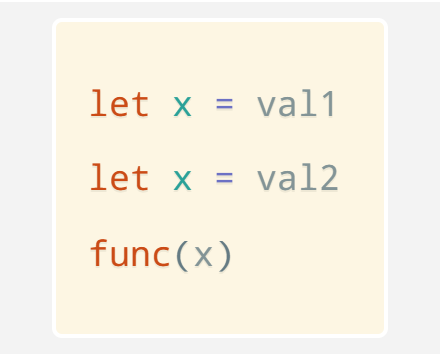
\includegraphics[width=0.9\linewidth, trim={0.2cm 0.2cm 0.2cm 0.2cm}, clip]{figs/let.png}
\captionof{figure}{\color{DarkRed} $let$ in $DDecl$}
\end{center}
\end{minipage}

\begin{minipage}[b]{1\linewidth}
\begin{center}
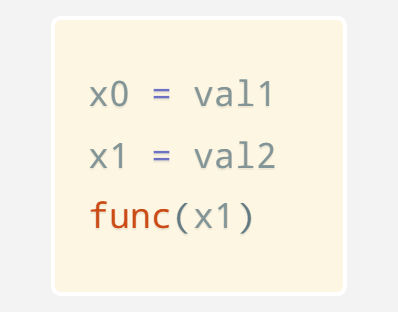
\includegraphics[width=0.9\linewidth, trim={0.2cm 0.3cm 0.2cm 0.2cm}, clip]{figs/let-by-mangling.png}
\captionof{figure}{\color{DarkRed} Eliminating $let$ by name mangling}
\end{center}
\end{minipage}


\begin{minipage}[b]{1\linewidth}
\begin{center}
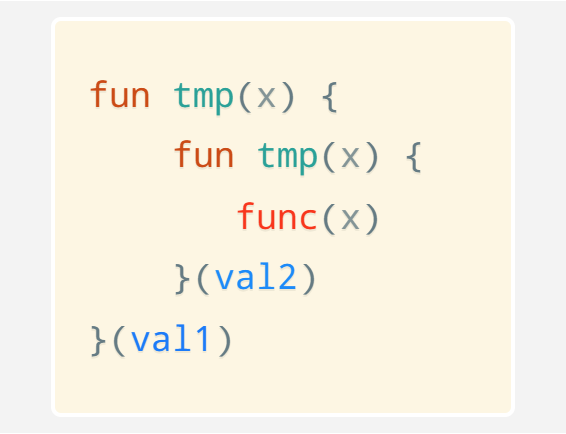
\includegraphics[width=0.9\linewidth, trim={0.2cm 0.2cm 0.2cm 0.3cm}, clip]{figs/let-by-im-call.png}
\vspace{-0.65cm}
\captionof{figure}{\color{DarkRed} Eliminating $let$ by immediately invoked functions(abbr. IIFE)}
\end{center}
\end{minipage}
\end{multicols}

\vspace{-1cm}

\begin{multicols}{2}

\begin{minipage}[b]{1\linewidth}
\begin{center}\vspace{0.1cm}
    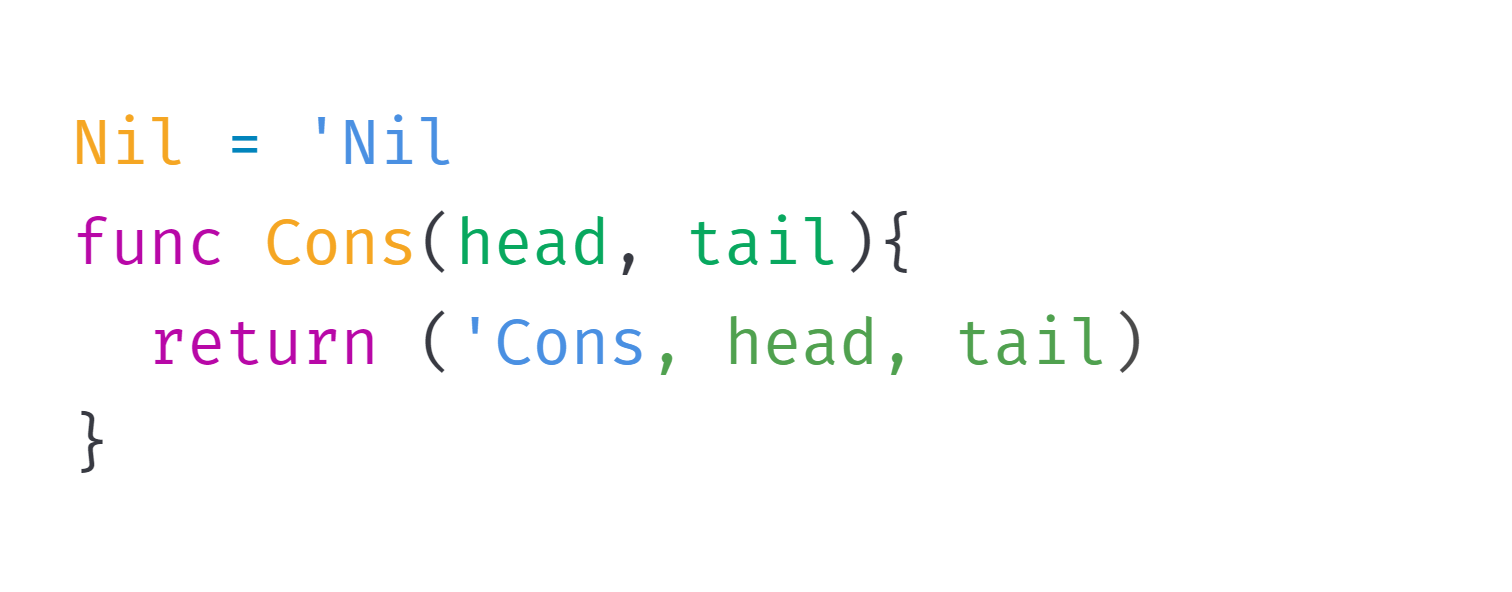
\includegraphics[width=1\linewidth, trim={0.1cm 0.1cm 0.1cm 0.1cm}, clip]{figs/tagged-union-impl.png}
    \vspace{-1.5cm}
    \captionof{figure}{\color{DarkRed} ADT internals in back ends}
\end{center}
\end{minipage}


\begin{minipage}[b]{1\linewidth}
\begin{center}\vspace{0.75cm}
    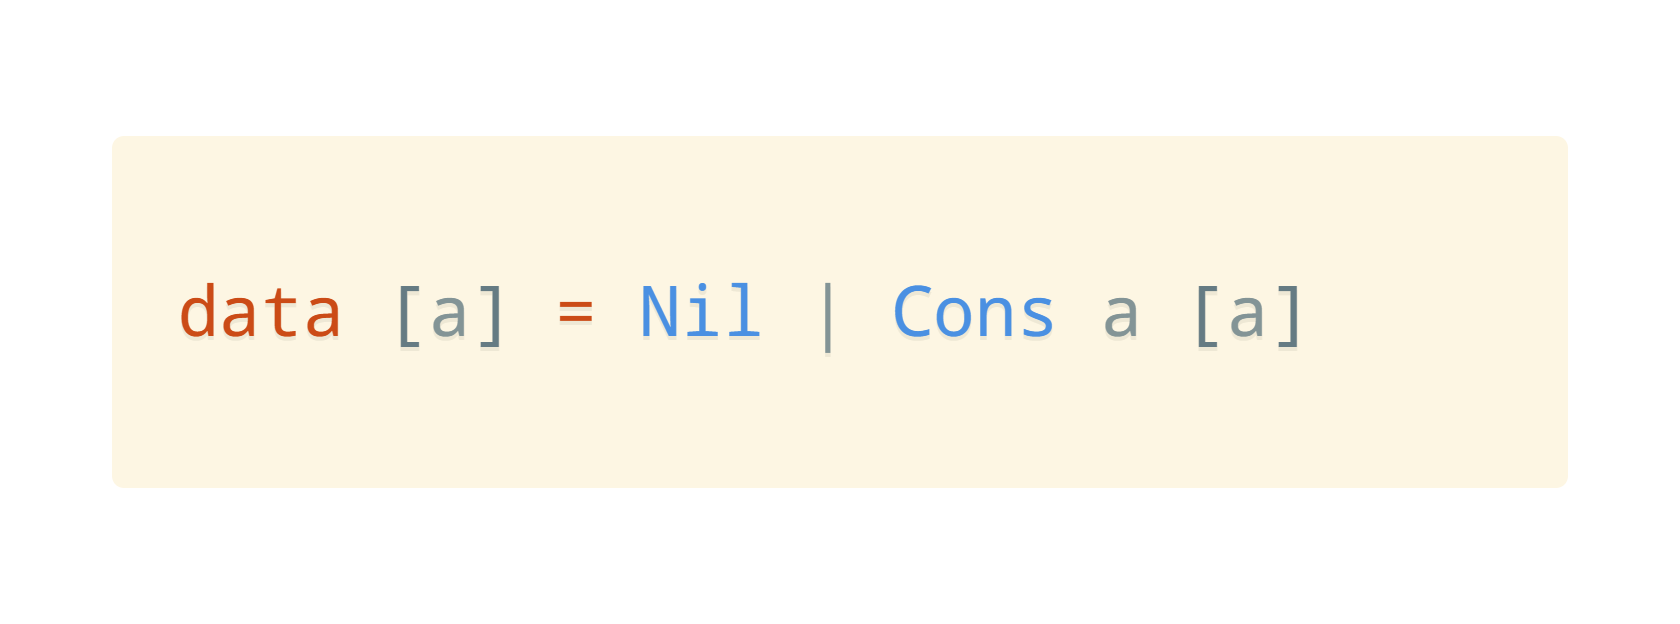
\includegraphics[width=1\linewidth, trim={0.2cm 0.2cm 0.2cm 0.3cm}, clip]{figs/tagged-union.png}
    \vspace{-1.5cm}
    \captionof{figure}{\color{DarkRed} Algebraic Data Types(ADTs)}
\end{center}
\end{minipage}

\end{multicols}

Other than above desugaring and lowering, $DDecl$ is still tough to tackle as back end implementer
should aware various primitive operations and constructs, such as
projections $Proj$, FFIs $Foreign$, throwing exceptions $Error$, and primitive operators $Op$.

It could be beneficial to transfer the complexity to the upstream, i.e., a runtime system of
the back end \cite {appel1990runtime}, see \textbf{table 1}, columns \textbf{DDecl} and \textbf{JavaScript-like pseudo code}.

\begin{center}
\begin{tabular}{ |c|c|c|c| } 
 \toprule
 \textit{Cases} & \textit{DDecl} & \textit{JavaScript-like pseudo code} & \textit{WDecl}\\
 \midrule
 Integer Additions & \tbcell{figs/cell-1-1.png} & \tbcell[0.25]{figs/cell-1-2.png} & \tbcell[0.25]{figs/cell-1-3.png}\\
 \midrule
 Projections & \tbcell[0.15]{figs/cell-2-1.png} & \tbcell[0.23]{figs/cell-2-2.png} & \tbcell[0.25]{figs/cell-2-3.png} \\
 \midrule
 Pattern Matching 1 & \tbcell{figs/cell-3-1.png} & \tbcell[0.25]{figs/cell-3-2.png} & ... \\
 \midrule
 Pattern Matching 2 & \tbcell{figs/cell-4-1.png} & \tbcell[0.25]{figs/cell-4-2.png} & ... \\
 \midrule
 Construction 1 & \tbcell[0.15]{figs/cell-5-1.png} & \tbcell[0.09]{figs/cell-5-2.png} & \tbcell[0.25]{figs/cell-5-3.png} \\
 \midrule
 Construction 2 & \tbcell{figs/cell-6-1.png} & \tbcell[0.25]{figs/cell-6-2.png} & ... \\
 \bottomrule
\end{tabular}
\captionof{table}{\color{DarkRed} Correspondences}
\end{center}


% We also have to

% \begin{itemize}
%     \setlength\itemsep{-0.1em}
%     \item translate pattern matching things to non-pattern match languages
%     \item translate block expressions \cite{gcc-stmt-expr} \cite{pep572} into languages whose expressions cannot accommodate statements
%     \item support primitive operations
%     \item support FFI
% \end{itemize}

% Options shall be provided here to control the properties of the IR, to achieve the reuse of
% \begin{itemize}
%     \setlength\itemsep{-0.2em}
%     \item desugaring block expressions, which may requires register allocation optimisations.
%     \item  desugaring pattern matching to switch statements and if statements
%     \item  desugaring data constructors to normal functions
%     \item  using LISP-style $Symbol$ as the tag of tagged union, for a language with $Symbol$ data.
%     \item  emulation of $Symbol$ in the language without $Symbol$ data for tags of tagged unions
% \end{itemize}

% Those stuffs are not difficult, but quite annoying when implementing
% them again and again, for each back end.

\section*{Proposal}

To address problems mentioned in section $Investigation$, We hereby propose a new IR,
which is lightweight, neat and compact, and finally capable of getting used to implement a back end reasonably fast.


\vspace{-1.5cm}
\begin{multicols}{2}

\begin{minipage}[t]{0.8\linewidth}
\begin{bnf*}
    \bnfprod{block-stmt}{\bnfts{[} \bnftd{stmt}\bnfts{]}}\\
    \bnfprod{stmt}{\bnftd{Intro} \bnfsp \bnftd{name}}\\
    \bnfmore{\bnfor \bnftd{Up} \bnfsp \bnftd{name} \bnfsp \bnftd{expr}}\\
    \bnfmore{\bnfor \bnftd{If} \bnfsp \bnftd{expr} \bnfsp \bnftd{block-stmt} \bnfsp \bnftd{block-stmt}}\\
    \bnfmore{\bnfor \bnftd{Eff} \bnfsp \bnftd{expr}}\\
    \bnfmore{\bnfor \bnftd{Ret} \bnfsp \bnftd{expr}}\\
    \bnfmore{\bnfor \bnftd{Switch} \bnfsp \bnftd{expr} \bnfsp \bnfts{[} \bnftd{(} \bnfsp \bnftd{constant} \bnfsp \bnftd{,} \bnfsp \bnftd{block-stmt} \bnfsp \bnftd{)}\bnfts{]} \bnfsp \bnftd{block-stmt}}\\
\end{bnf*}
\end{minipage}

\vfill\null
\columnbreak

\begin{minipage}[t]{0.8\linewidth}
\begin{bnf*}
    \bnfprod{ext}{\bnftd{ExtApp} \bnfsp \bnftd{name} \bnfsp \bnfts{[} \bnftd{expr} \bnfts{]} }\\
    \bnfmore{\bnfor \bnftd{ExtVar} \bnfsp \bnftd{name}}\\
    \bnfprod{expr}{\bnftd{Var} \bnfsp \bnftd{name}}\\
    \bnfmore{\bnfor \bnftd{App} \bnfsp \bnftd{name} \bnfsp \bnfts{[} \bnftd{expr}\bnfts{]}}\\
    \bnfmore{\bnfor \bnftd{Const} \bnfsp \bnftd{constant-literal}}\\
    \bnfmore{\bnfor \bnftd{Ext} \bnfsp \bnftd{ext}}\\
\end{bnf*}
\end{minipage}
\end{multicols}

\vspace{-1cm}

\begin{center} {\textbf{Language 2}: \color{DarkRed} \textbf{Weakest Declarations}} \end{center}

Instead of leaving a blank for the internal implementations of product types, FFIs, constructors of algebraic data,
we can assume a generally applicable implementation for each of them, and finally,
transform $DDecl$ to the proposed IR, with desugaring $Let$ expressions and block expressions, and permitting
optional transformations which might be required by some back ends.

We'd call it a \textbf{Weakest Declaration}(abbr. $WDecl$), as it is weak enough to be expressed by
all of the target programming languages investigated in this project.

See \text{Table 1} for the correspondences between $DDecl$, JavaScript-like pseudo code, and $WDecl$.

\color{FireBrick} %  colour for the conclusions to make them stand out

\section*{Results}

We implemented the transformation from $DDecl$ to $WDecl$ in the Haskell side,
then produced a binary executable which compiles Idris source files to a standalone \textbf{.qb} file.

A target language will later read $WDecl$ IR from the \textbf{.qb} file,
and then do back end specific code generation, i.e., Haskell side
is not responsible for generating executable code from Idris source files.

This strategy is advantageous,
as most long-living languages have their own libraries or features
to idiomatically manipulate their own programs as data.

Finally, we provided back end implementations for Python, Julia, Ruby and Erlang,
with a surprisingly concise code, each of which consists of only
trivial procedures within a sparse 200 lines,
and tested by the examples provided by official website of Idris tutorials.

\begin{center}
\begin{tabular}{ |c|c|c|c } 
 \toprule
 \textit{Target Language} & \textit{Existing Implementation, Line Count} & \textit{Line Count by QB(abbr. Quick Backend)} & \textit{Notes} \\
 \midrule
 Python2 & ziman/idris-py, $> 900$ & 177 & QB: Python 2+3 \\
 Python3 & thautwarm/idris-python, $> 1000$ & 177 & ditto \\
 Ruby & mrb/idris-ruby, $> 220 $ &  209 & QB: full-featured + optimized \\
 Julia & none so far & 171 & very fast \\
 \bottomrule
\end{tabular}
\captionof{table}{\color{DarkRed} Line count comparisons of results}
\end{center}

Note that, by using our Quick Backend implementation, a lot of stuffs
such as FFI, primitive operations get decoupled from the back end implementation itself,
as a result, we gain extensibility,
and further optimizations can be easily introduced as plugins.

TODO: add erlang backend and JavaScript backend tonight

\section*{Conclusions}

We achieved our goal of implementing Idris back ends quickly, with the capability of reusing transformations used by multiple back ends.


\begin{multicols}{2}

\begin{minipage}[t]{0.9\linewidth}
Some reusable transformations:
\begin{itemize}
    \setlength\itemsep{-0.2em}
    \item LISP-symbol emulations
    \item arbitrary identifier to the classic Java identifier
    \item block expression desugaring
    \item let expression desugaring
    \item pattern matching compilation
\end{itemize}
\end{minipage}

\begin{minipage}[t]{0.8\linewidth}
Due to the limitations of our bandwidth, the more difficult transformations are missing.
However, it shall not be a problem, as what matters here is how to reuse of transformations for multiple back ends.

\begin{itemize}
    \setlength\itemsep{-0.2em}
    \item tail call scheduling
    \item register allocation optimizations
    \item mutation to state monads
\end{itemize}
\end{minipage}

\end{multicols}

\vspace{-1cm}

\color{Black}

\section*{Forthcoming Research}

Although Idris is powerful enough to express very complex static properties,
there're still cases where runtime checking will be needed.

Some reasons here could be

\begin{itemize}
    \setlength\itemsep{-0.2em}
    \item Constructing proofs for complex properties is pretty niche, requiring specific and knowledge about dependent types and theorem proving.
    \item Programmers incapable of prove the correctness with their code, might be able to prove it in other means.
    \item Idris itself is not perfect enough to prove things just like as is, i.e., hand-written mathematical proofs can sometimes be easier.
\end{itemize}

To support runtime checking, the reasonable error reports and debugging shall be supported,
which both require some metadata from the original source code, e.g.,

\begin{itemize}
    \setlength\itemsep{-0.2em}
    \item filename
    \item source line number
    \item source column number
\end{itemize}

All these metadata are missing in $DDecl$ or other convenient IRs provided by Idris,
as a consequence, it's impossible to get a practical runtime checking.


\section*{Acknowledgements}

Archibald Samuel Elliott for his elaborated notes about Idris $DDecl$ \cite {elliott2015concurrency}, and so far all those IRs are highly-undocumented in Idris official site.

\begin{small}%Makes the text of the references section smaller
\begin{multicols}{2}%Makes the section two col
\nocite{*} % Print all references regardless of whether they were cited in the poster or not
\bibliographystyle{plain} % Plain referencing style
\bibliography{bibliography} % Use the example bibliography file sample.bib
\end{multicols}
\end{small}


% \section*{Supplementary}

% $WDecl$ is actually simpler than the so-called $SDecl$ provided by the Idris compiler \cite {brady2013idris} as their simplest IR.

% The reason why we take $WDecl$ as the weakest is, incidentally, it's like a simplified form
% of ASTs of the Python Programming Language.
% Python is the weakest programming language among all well-known dynamic programming languages,
% which is to say, despite of the details of object models/systems, Python can be trivially
% expressed/translated to Ruby, Lua, JavaScript, Erlang, etc., whereas transforming
% from the latter ones to Python is thorny, due to the lack of block expressions and
% assignment expressions \cite {pep572}. Although the weakness of Python is considered harmful in regular
% programming tasks, it unveils what a generally transformable upstream IR shall look like.

\end{multicols}

\end{document}

